% Copyright 2006 by Till Tantau
%
% This file may be distributed and/or modified
%
% 1. under the LaTeX Project Public License and/or
% 2. under the GNU Free Documentation License.
%
% See the file doc/generic/pgf/licenses/LICENSE for more details.

\section{Transformations}

\pgfname\ has a powerful transformation mechanism that is similar to
the transformation capabilities of \textsc{metafont}. The present
section explains how you can access it in \tikzname.


\subsection{The Different Coordinate Systems}

It is a long process from  a coordinate like, say, $(1,2)$ or
$(1\mathrm{cm},5\mathrm{pt})$, to the position a point is finally
placed on the display or paper. In order to find out where the point
should go, it is constantly ``transformed,'' which means that it is
mostly shifted around and possibly rotated, slanted, scaled, and
otherwise mutilated.

In detail, (at least) the following transformations are applied to a
coordinate like $(1,2)$ before a point on the screen is chosen:
\begin{enumerate}
\item
  \pgfname\ interprets a coordinate like $(1,2)$  in its
  $xy$-coordinate system as ``add the current $x$-vector once and the
  current $y$-vector twice to obtain the new point.''
\item
  \pgfname\ applies its coordinate transformation matrix to the
  resulting coordinate. This yields the final position of the point
  inside the picture.
\item
  The backend driver (like |dvips| or |pdftex|) adds transformation
  commands such the coordinate is shifted to the correct position in
  \TeX's page coordinate system.
\item
  \textsc{pdf} (or PostScript) apply the canvas transformation
  matrix to the point, which can once more change the position on the
  page.
\item
  The viewer application or the printer applies the device
  transformation matrix to transform the coordinate to its final pixel
  coordinate on the screen or paper.
\end{enumerate}

In reality, the process is even more involved, but the above should
give the idea: A point is constantly transformed by changes of the
coordinate system.

In \tikzname, you only have access to the first two coordinate systems:
The $xy$-coordinate system and the coordinate transformation matrix
(these will be explained later). \pgfname\ also allows you to change
the canvas transformation matrix, but you have to use commands of
the core layer directly to do so and you ``better know what you are
doing'' when you do this. The moment you start modifying the
canvas matrix, \pgfname\ immediately looses track of all
coordinates and shapes, anchors, and bounding box computations will no
longer work.


\subsection{The XY- and XYZ-Coordinate Systems}
\label{section-xyz}

The first and easiest coordinate systems are \pgfname's $xy$- and
$xyz$-coordinate systems. The idea is very simple: Whenever you
specify a coordinate like |(2,3)| this means $2v_x + 3v_y$, where
$v_x$ is the current \emph{$x$-vector} and $v_y$ is the current
\emph{$y$-vector}. Similarly, the coordinate |(1,2,3)| means $v_x +
2v_y + 3v_z$.

Unlike other packages, \pgfname\ does not insist that $v_x$ actually
has a $y$-component of $0$, that is, that it is a horizontal
vector. Instead, the $x$-vector can point anywhere you
want. Naturally, \emph{normally} you will want the $x$-vector to point
horizontally.

One undesirable effect of this flexibility is that it is not possible
to provide mixed coordinates as in $(1,2\mathrm{pt})$. Life is hard.

To change the $x$-, $y$-, and $z$-vectors, you can use the following
options:

\begin{key}{/tikz/x=\meta{value} (initially 1cm)}
  If \meta{value} is a dimension, the $x$-vector of
  \pgfname's $xyz$-coordinate system is setup to point
  \meta{value} to the right, that is, to $(\meta{value},0pt)$.

\begin{codeexample}[]
\begin{tikzpicture}
  \draw                  (0,0)   -- +(1,0);
  \draw[x=2cm,color=red] (0,0.1) -- +(1,0);
\end{tikzpicture}
\end{codeexample}

\begin{codeexample}[]
\tikz \draw[x=1.5cm] (0,0) grid (2,2);
\end{codeexample}

  The last example shows that the size of steppings in grids, just like
  all other dimensions, are not affected by the $x$-vector. After all,
  the $x$-vector is only used to determine the coordinate of the upper
  right corner of the grid.

  If \meta{value} is a coordinate, the $x$-vector of
  \pgfname's $xyz$-coordinate system to the specified coordinate. If
  \meta{value} contains a comma, it must be put in braces.

\begin{codeexample}[]
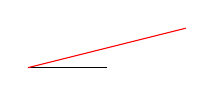
\begin{tikzpicture}
  \draw                            (0,0) -- (1,0);
  \draw[x={(2cm,0.5cm)},color=red] (0,0) -- (1,0);
\end{tikzpicture}
\end{codeexample}

  You can use this, for example, to exchange the meaning of the $x$- and
  $y$-coordinate.

\begin{codeexample}[]
\begin{tikzpicture}[smooth]
  \draw plot coordinates{(1,0) (2,0.5) (3,0) (3,1)};
  \draw[x={(0cm,1cm)},y={(1cm,0cm)},color=red]
        plot coordinates{(1,0) (2,0.5) (3,0) (3,1)};
\end{tikzpicture}
\end{codeexample}
\end{key}

\begin{key}{/tikz/y=\meta{value} (initially 1cm)}
  Works like the |x=| option, only if \meta{value} is a dimension, the
  resulting vector points to $(0,\meta{value})$.
\end{key}

\begin{key}{/tikz/z=\meta{value} (initially \normalfont$-3.85$mm)}
  Works like the |y=| option, but now a dimension is means the point
  $(\meta{value},\meta{value})$.

\begin{codeexample}[]
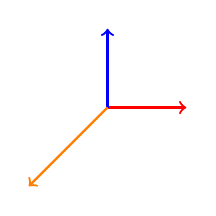
\begin{tikzpicture}[z=-1cm,->,thick]
  \draw[color=red] (0,0,0) -- (1,0,0);
  \draw[color=blue] (0,0,0) -- (0,1,0);
  \draw[color=orange] (0,0,0) -- (0,0,1);
\end{tikzpicture}
\end{codeexample}
\end{key}



\subsection{Coordinate Transformations}

\pgfname\ and \tikzname\ allow you to specify \emph{coordinate
  transformations}. Whenever you specify a coordinate as in |(1,0)| or
|(1cm,1pt)| or |(30:2cm)|, this coordinate is first
``reduced'' to a position of the form ``$x$ points to the right and
  $y$ points upwards.'' For example, |(1in,5pt)| is reduced to
``$72\frac{72}{100}$ points to the right and 5 points upwards'' and
|(90:100pt)| means ``0pt to the right and 100 points upwards.''

The next step is to apply the current \emph{coordinate transformation
  matrix} to the coordinate. For example, the coordinate
transformation matrix might currently be set such that it adds a
certain constant to the $x$ value. Also, it might be setup such that
it, say, exchanges the $x$ and $y$ value. In general, any
``standard'' transformation like translation, rotation, slanting, or
scaling or any combination thereof is possible. (Internally, \pgfname\
keeps track of a coordinate transformation matrix very much like the
concatenation matrix used by \textsc{pdf} or PostScript.)

\begin{codeexample}[]
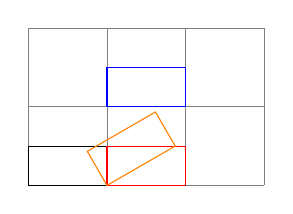
\begin{tikzpicture}
  \draw[help lines] (0,0) grid (3,2);
  \draw (0,0) rectangle (1,0.5);
  \begin{scope}[xshift=1cm]
    \draw             [red]    (0,0) rectangle (1,0.5);
    \draw[yshift=1cm] [blue]   (0,0) rectangle (1,0.5);
    \draw[rotate=30]  [orange] (0,0) rectangle (1,0.5);
  \end{scope}
\end{tikzpicture}
\end{codeexample}

The most important aspect of the coordinate transformation matrix is
\emph{that it applies to coordinates only!} In particular, the
coordinate transformation has no effect on things like the line width
or the dash pattern or the shading angle. In certain cases, it is not
immediately clear whether the coordinate transformation matrix
\emph{should} apply to a certain dimension. For example, should the
coordinate transformation matrix apply to grids? (It does.) And what
about the size of arced corners? (It does not.) The general rule is
``If there is no `coordinate' involved, even `indirectly,' the matrix
is not applied.'' However, sometimes, you simply have to try or look
it up in the documentation whether the matrix will be applied.

Setting the matrix cannot be done directly. Rather, all you can do is
to ``add'' another transformation to the current matrix. However, all
transformations are local to the current \TeX-group. All
transformations are added using graphic options, which are described
below.

Transformations apply immediately when they are encountered ``in the
middle of a path'' and they apply only to the coordinates on the path
following the transformation option.

\begin{codeexample}[]
\tikz \draw (0,0) rectangle (1,0.5) [xshift=2cm] (0,0) rectangle (1,0.5);
\end{codeexample}

A final word of warning: You should refrain from using ``aggressive''
transformations like a scaling of a factor of 10000. The reason is
that all transformations are done using \TeX, which has a fairly low
accuracy. Furthermore, in certain situations it is necessary that
\tikzname\ \emph{inverts} the current transformation matrix and this will
fail if the transformation matrix is badly conditioned or even
singular (if you do not know what singular matrices are, you are blessed).

\begin{key}{/tikz/shift={\ttfamily\char`\{}\meta{coordinate}{\ttfamily\char`\}}}
  Adds the \meta{coordinate} to all coordinates.
\begin{codeexample}[]
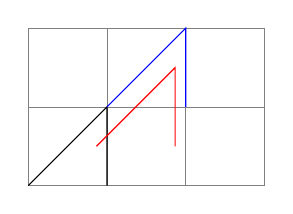
\begin{tikzpicture}
  \draw[help lines] (0,0) grid (3,2);
  \draw                       (0,0) -- (1,1) -- (1,0);
  \draw[shift={(1,1)},blue]   (0,0) -- (1,1) -- (1,0);
  \draw[shift={(30:1cm)},red] (0,0) -- (1,1) -- (1,0);
\end{tikzpicture}
\end{codeexample}
\end{key}

\begin{key}{/tikz/shift only}
  This option does not take any parameter. Its effect is to cancel all
  current transformations except for the shifting. This means that the
  origin will remain where it is, but any rotation around the origin
  or scaling relative to the origin or skewing will no longer have an
  effect.

  This option is useful in situations where a complicated
  transformation is used to ``get to a position,'' but you then wish
  to draw something ``normal'' at this position.

\begin{codeexample}[]
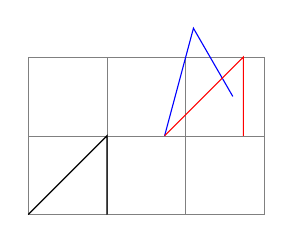
\begin{tikzpicture}
  \draw[help lines] (0,0) grid (3,2);
  \draw                                      (0,0) -- (1,1) -- (1,0);
  \draw[rotate=30,xshift=2cm,blue]           (0,0) -- (1,1) -- (1,0);
  \draw[rotate=30,xshift=2cm,shift only,red] (0,0) -- (1,1) -- (1,0);
\end{tikzpicture}
\end{codeexample}
\end{key}

\begin{key}{/tikz/xshift=\meta{dimension}}
  Adds \meta{dimension} to the $x$ value of all coordinates.
\begin{codeexample}[]
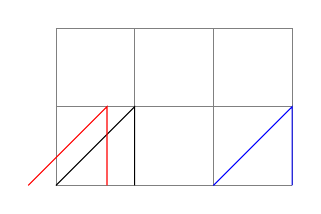
\begin{tikzpicture}
  \draw[help lines] (0,0) grid (3,2);
  \draw                   (0,0) -- (1,1) -- (1,0);
  \draw[xshift=2cm,blue]  (0,0) -- (1,1) -- (1,0);
  \draw[xshift=-10pt,red] (0,0) -- (1,1) -- (1,0);
\end{tikzpicture}
\end{codeexample}
\end{key}

\begin{key}{/tikz/yshift=\meta{dimension}}
  Adds \meta{dimension} to the $y$ value of all coordinates.
\end{key}

\begin{key}{/tikz/scale=\meta{factor}}
  Multiplies all coordinates by the given \meta{factor}. The
  \meta{factor} should not be excessively large in absolute terms or
  very near to zero.
\begin{codeexample}[]
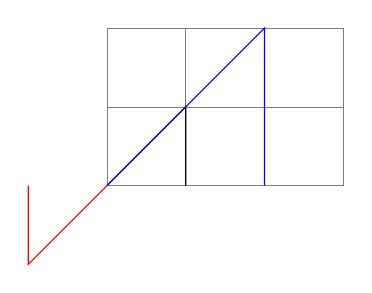
\begin{tikzpicture}
  \draw[help lines] (0,0) grid (3,2);
  \draw               (0,0) -- (1,1) -- (1,0);
  \draw[scale=2,blue] (0,0) -- (1,1) -- (1,0);
  \draw[scale=-1,red] (0,0) -- (1,1) -- (1,0);
\end{tikzpicture}
\end{codeexample}
\end{key}

\begin{key}{/tikz/scale around={\ttfamily\char`\{}\meta{factor}|:|\meta{coordinate}{\ttfamily\char`\}}}
  Scales the coordinate system by \meta{factor}, put with the ``origin
  of scaling'' centered on \meta{coordinate} rather than the origin.
\begin{codeexample}[]
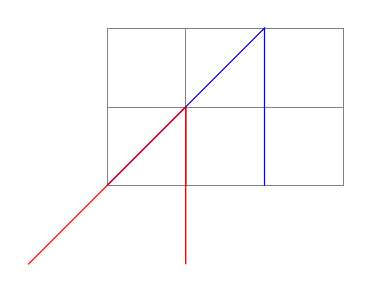
\begin{tikzpicture}
  \draw[help lines] (0,0) grid (3,2);
  \draw                             (0,0) -- (1,1) -- (1,0);
  \draw[scale=2,blue]               (0,0) -- (1,1) -- (1,0);
  \draw[scale around={2:(1,1)},red] (0,0) -- (1,1) -- (1,0);
\end{tikzpicture}
\end{codeexample}
\end{key}

\begin{key}{/tikz/xscale=\meta{factor}}
  Multiplies only the $x$-value of all coordinates by the given
  \meta{factor}.
\begin{codeexample}[]
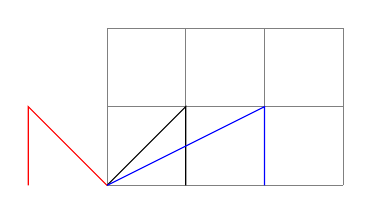
\begin{tikzpicture}
  \draw[help lines] (0,0) grid (3,2);
  \draw                (0,0) -- (1,1) -- (1,0);
  \draw[xscale=2,blue] (0,0) -- (1,1) -- (1,0);
  \draw[xscale=-1,red] (0,0) -- (1,1) -- (1,0);
\end{tikzpicture}
\end{codeexample}
\end{key}

\begin{key}{/tikz/yscale=\meta{factor}}
  Multiplies only the $y$-value of all coordinates by \meta{factor}.
\end{key}

\begin{key}{/tikz/xslant=\meta{factor}}
  Slants the coordinate horizontally by the given \meta{factor}:
\begin{codeexample}[]
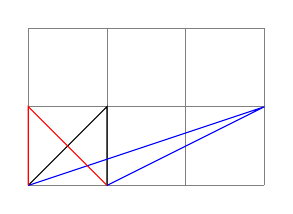
\begin{tikzpicture}
  \draw[help lines] (0,0) grid (3,2);
  \draw                (0,0) -- (1,1) -- (1,0);
  \draw[xslant=2,blue] (0,0) -- (1,1) -- (1,0);
  \draw[xslant=-1,red] (0,0) -- (1,1) -- (1,0);
\end{tikzpicture}
\end{codeexample}
\end{key}


\begin{key}{/tikz/yslant=\meta{factor}}
  Slants the coordinate vertically by the given \meta{factor}:
\begin{codeexample}[]
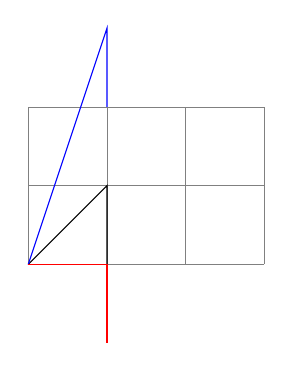
\begin{tikzpicture}
  \draw[help lines] (0,0) grid (3,2);
  \draw                (0,0) -- (1,1) -- (1,0);
  \draw[yslant=2,blue] (0,0) -- (1,1) -- (1,0);
  \draw[yslant=-1,red] (0,0) -- (1,1) -- (1,0);
\end{tikzpicture}
\end{codeexample}
\end{key}


\begin{key}{/tikz/rotate=\meta{degree}}
  Rotates the coordinate system by \meta{degree}:
\begin{codeexample}[]
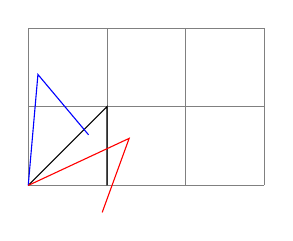
\begin{tikzpicture}
  \draw[help lines] (0,0) grid (3,2);
  \draw                 (0,0) -- (1,1) -- (1,0);
  \draw[rotate=40,blue] (0,0) -- (1,1) -- (1,0);
  \draw[rotate=-20,red] (0,0) -- (1,1) -- (1,0);
\end{tikzpicture}
\end{codeexample}
\end{key}

\begin{key}{/tikz/rotate around={\ttfamily\char`\{}\meta{degree}|:|\meta{coordinate}{\ttfamily\char`\}}}
  Rotates the coordinate system by \meta{degree} around the point
  \meta{coordinate}.
\begin{codeexample}[]
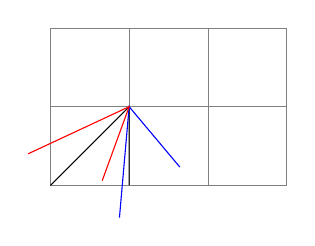
\begin{tikzpicture}
  \draw[help lines] (0,0) grid (3,2);
  \draw                                (0,0) -- (1,1) -- (1,0);
  \draw[rotate around={40:(1,1)},blue] (0,0) -- (1,1) -- (1,0);
  \draw[rotate around={-20:(1,1)},red] (0,0) -- (1,1) -- (1,0);
\end{tikzpicture}
\end{codeexample}
\end{key}


\begin{key}{/tikz/cm={\ttfamily\char`\{}\meta{$a$}|,|\meta{$b$}|,|\meta{$c$}|,|\meta{$d$}|,|\meta{coordinate}{\ttfamily\char`\}}}
  applies the following transformation to all coordinates: Let $(x,y)$
  be the coordinate to be transformed and let \meta{coordinate}
  specify the point $(t_x,t_y)$. Then the new coordinate is given by
  $\left(\begin{smallmatrix} a & b \\ c & d\end{smallmatrix}\right)
  \left(\begin{smallmatrix} x \\ y \end{smallmatrix}\right) +
  \left(\begin{smallmatrix} t_x \\ t_y
  \end{smallmatrix}\right)$. Usually, you do not use this option
  directly.
\begin{codeexample}[]
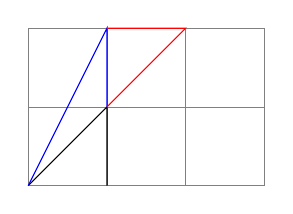
\begin{tikzpicture}
  \draw[help lines] (0,0) grid (3,2);
  \draw                             (0,0) -- (1,1) -- (1,0);
  \draw[cm={1,1,0,1,(0,0)},blue]    (0,0) -- (1,1) -- (1,0);
  \draw[cm={0,1,1,0,(1cm,1cm)},red] (0,0) -- (1,1) -- (1,0);
\end{tikzpicture}
\end{codeexample}
\end{key}

\begin{key}{/tikz/reset cm}
  Completely resets the coordinate transformation matrix to the
  identity matrix. This will destroy not only the transformations
  applied in the current scope, but also all transformations inherited
  from surrounding scopes. Do not use this option, unless you really,
  really know what you are doing.
\end{key}




\subsection{Canvas Transformations}

A \emph{canvas transformation}, see
Section~\ref{section-design-transformations} for details, is best
thought of as a transformation in which the drawing canvas is
stretched or rotated. Imaging writing something on a balloon (the
canvas) and then blowing air into the balloon: Not only does the text
become larger, the thin lines also become larger. In particular, if
you scale the canvas by a factor of two, all lines are twice as
thick.

Canvas transformations should be used with great care. In most
circumstances you do \emph{not} want line widths to change in a
picture as this creates visual inconsistency.

Just as important, when
you use canvas transformations \emph{\pgfname\ looses track of
  positions of nodes and of picture sizes} since it does not take the
effect of canvas transformations into account when it computes
coordinates of nodes (you not, however, rely on this; it may change in
the future).

Finally, not that a canvas transformation always applies to a path as
a whole, it is not possible (as for coordinate transformations) to use
different transformations in different parts of a path.

In short, you should not use canvas transformations unless you really
know what you are doing.

\begin{key}{/tikz/transform canvas=\meta{options}}
  The \meta{options} should contain coordinate transformations options
  like |scale| or |xshift|. Multiple options can be given, their
  effects accumulate in the usual manner. The effect of these
  \meta{options} (immediately) changes the current canvas
  transformation matrix. The coordinate transformation matrix is not
  changed. Tracking of the picture size is (locally) switched off and
  the node coordinate will no longer be correct.
\begin{codeexample}[]
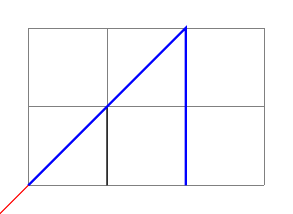
\begin{tikzpicture}
  \draw[help lines] (0,0) grid (3,2);
  \draw                                    (0,0) -- (1,1) -- (1,0);
  \draw[transform canvas={scale=2},blue]   (0,0) -- (1,1) -- (1,0);
  \draw[transform canvas={rotate=180},red] (0,0) -- (1,1) -- (1,0);
\end{tikzpicture}
\end{codeexample}
\end{key}
